\documentclass[UTF8]{ctexart}
\usepackage{graphicx}
\usepackage[T1]{fontenc}
\usepackage{charter}
\usepackage{amsmath}
\usepackage{amssymb}
\usepackage{listings}
\usepackage{color}
\usepackage{xcolor}
\usepackage{hyperref}
\usepackage{booktabs}
\usepackage{tabularx}
\usepackage{geometry}
\usepackage{float}

\geometry{a4paper,left=2cm,right=2cm,top=2cm,bottom=2cm}

\title{\heiti SpinalHDL 编写的打地鼠游戏}
\author{\kaishu 张政镒 \quad 20300750021}
\date{\today}


\definecolor{codegreen}{rgb}{0,0.6,0}
\definecolor{wasurenagusa}{rgb}{0.54, 0.76, 0.92}
\definecolor{ruri}{rgb}{0.12, 0.31, 0.63}
\definecolor{codegray}{rgb}{0.5,0.5,0.5}
\definecolor{codepurple}{rgb}{0.58,0,0.82}
\definecolor{backcolor}{rgb}{0.97,0.98,0.99}
\lstset{
        backgroundcolor=\color{backcolor},   
        commentstyle=\color{ruri},
        keywordstyle=\color{magenta},
        numberstyle=\tiny\color{codegray},
        stringstyle=\color{codepurple},
        basicstyle=\small\ttfamily,
        breakatwhitespace=false,         
        breaklines=true,
        captionpos=b,   
        frame=shadowbox,                 
        keepspaces=true,                 
        numbers=left,                    
        numbersep=10pt,                  
        showspaces=false,                
        showstringspaces=false,
        showtabs=false, 
        tabsize=2,        
}

\begin{document}
\maketitle
\tableofcontents

\section{设计规划}

\subsection{设计要求}

\subsubsection{设计内容}

设计一个打地鼠游戏机. 本设计在原题要求上进行了一定的扩展, 使得游戏机具有更好的可玩性. 下面是本设计的主要功能:

\begin{itemize}
    \item 用 HDMI 显示地鼠, 当前的难度以及得分情况.
    \item 有一个 Start 按钮用于控制游戏开始, 一个 Reset 按钮用于重置游戏.
    \item 游戏开始后, 会在屏幕上显示地鼠, 地鼠间隔一定的随机时间 $T_1$ 刷新位置并显示, 并持续 $T_2$ (随难度变化)时间. 
    \item 游戏分为 3 轮, 每轮游戏结束后若超过规定分数, 则进入下一轮. 在每轮游戏中, 打到地鼠得到的分数随难度增加而增加.
    \item 游戏结束后, 显示总分. 
\end{itemize}

\subsection{设计思路}

\subsubsection{硬件设计}

我采用 SpinalHDL 完成硬件设计部分. SpinalHDL 是一种基于 Scala 的硬件描述语言, 
可以生成 VHDL 或 Verilog 文件, 以此与现有的 EDA 工具兼容. 借由 Scala 提供的现代高级
编程语言的特性, SpinalHDL 可以大大提高硬件设计的效率. 它\textbf{不是}一种高层次综合语言, 
也非基于事件驱动的范式. 它依然是一种基于寄存器传输级 (RTL) 的描述范式. 

我采用 SpianlHDL 的原因在于其适用于快速开发迭代流程, 并提供良好的封装和代码可读性. 可以将
各个组件低耦合地设计, 并在最后组合起来. 它还提供了强大的参数化设计能力, 而这一点是在 Verilog
中很难做到的. 

\lstinputlisting[language=scala, caption={SpinalHDL 实现的加法器}, label={code:spinalexample}]{res/code/exampleOfSpinal.scala}

如代码\ref{code:spinalexample} 所示是一个简单的 SpinalHDL 示例, 其实现了一个位宽参数化的加法器. 



\subsubsection{软件仿真}

我使用了 Verilator 作为基本仿真工具并结合 Qt 作为图形化界面. 
Verilator 是一个开源的 Verilog仿真器, 它可以将 Verilog 代码编译成 C++ 代码, 并提供了一套 C++ API 用于仿真. 其优点在于
仿真速度快, 且可以方便地与 C++ 代码进行交互. Qt 是一个跨平台的 GUI 库, 可以方便地实现图形化界面. 通过
读取 Verilator 生成的仿真结果, 我可以在 C++ 中读取每一个周期的 RGB, VSYNC, HSYNC 信号, 并将其进行拼接, 
最终在软件端模拟一个显示器进行显示. 仿真器如图 \ref{fig:emulator} 所示. 

\begin{figure}
    \centering
    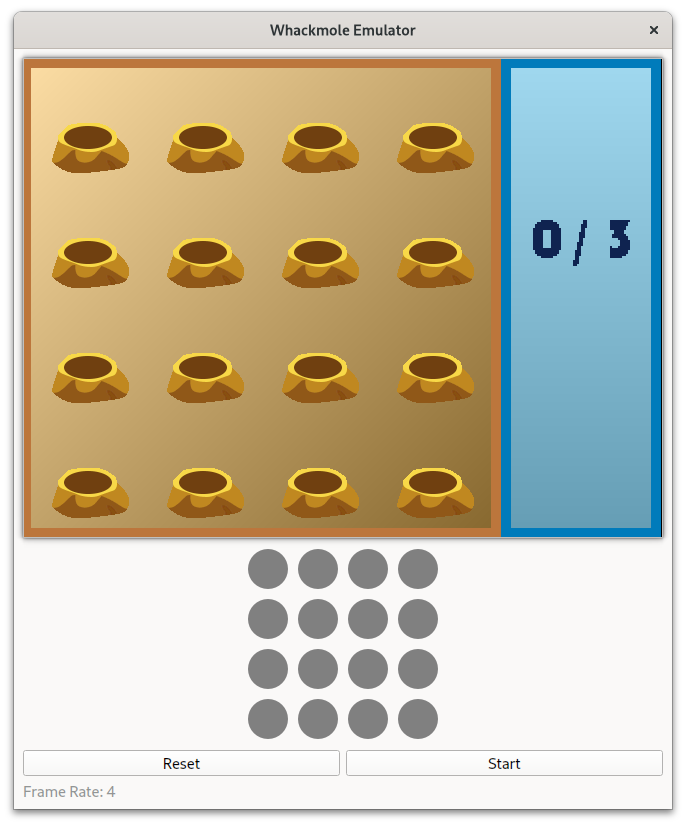
\includegraphics[width=0.5\textwidth]{res/img/emulator.png}
    \caption{以 Verilator 为基础的软件仿真器}
    \label{fig:emulator}
\end{figure}

显然, 软件端的模拟不可能达到硬件端的速度. 我采用的是640x480的分辨率, 以 60Hz 的刷新率进行显示的时序. 然而, 
软件端只能做到以 10Hz 的刷新率进行显示. 为了保证软件运行的稳定性(过高的刷新率容易导致处理跟不上, 从而使得
跨线程信号堆积), 我把软件的刷新率固定在了 5Hz. 那么, 我们怎么保证在时钟频率不同的硬件端和软件端游戏体验一致呢? 

好在, SpinalHDL 为我们提供了一套封装, 让我可以使用"秒"和"频率"作为参数进行设计. 如代码 \ref{code:spinaltime} 所示. 
这段代码是我实际使用的代码. 

\begin{lstlisting}[caption={SpinalHDL 中的时间参数}, label={code:spinaltime}, language=scala]
val frequency: HertzNumber = 2 MHz,
val roundGapTime: TimeNumber = 3 sec,
\end{lstlisting}

我向软件端传输的是 VGA 信号, 则刷新一帧需要 $525 \times 800 = 420000$ 个周期. 在 2 MHz 的
像素时钟下, 一帧需要 $420000 / 2000000 = 0.21$ 秒. 这样就能适应软件端 5 Hz 的刷新率.

如果要在硬件端实现, 我只需要将 2 MHz 改变为标准时钟频率 25.175 MHz 即可. 所有的时间参数, 例如
各轮之间的时长都不需要做任何额外的代码修改就能保持一致. 

\subsection{设计流程图及 EDA 使用说明}

设计流程图如图 \ref{fig:flowpath} 所示.

\begin{figure}
    \centering
    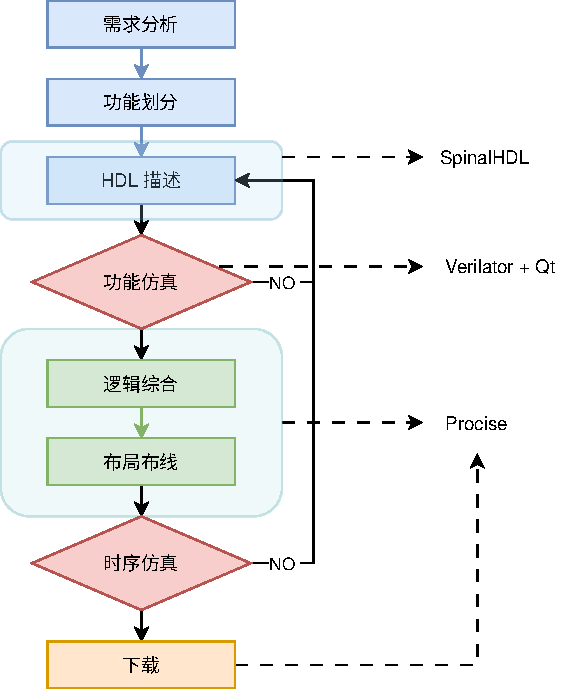
\includegraphics[width=0.5\textwidth]{res/img/flowpath.pdf}
    \caption{Top--Down 设计流程图}
    \label{fig:flowpath}
\end{figure}

本次设计的 FPGA 上板验证采用复微开发的 FPGA 开发板. 我也使用了 Procise 作为 EDA 工具进行综合和布局布线.

课程提供的工程示例对我帮助很大. 我在其基础上学习使用了 Procise 工具的使用方法, 掌握了该 EDA 工具的使用流程. 

\section{设计实现}

\subsection{框图介绍}

如图 \ref{fig:arch} 所示为游戏的框图. 下对框图进行简单介绍. 

\begin{figure}[htbp]
    \centering
    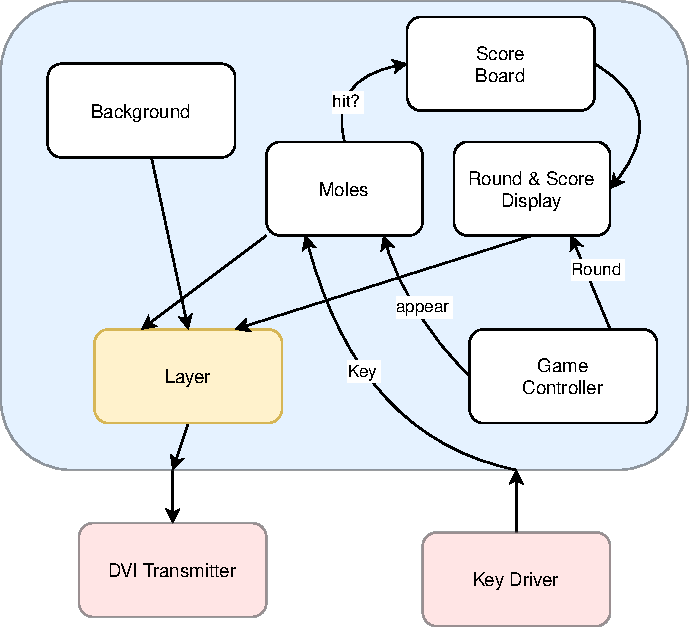
\includegraphics[width=0.7\textwidth]{res/img/arch.pdf}
    \caption{打地鼠游戏框图}
    \label{fig:arch}
\end{figure}

蓝色框图内部分是我自己设计的模块, 外面的 DVI Transmitter 以及 Key Driver 
来源于课程中提供的示例. 下对\textbf{蓝色框图内}的部分进行简单介绍. 

\begin{itemize}
    \item Moles: 地鼠. 该模块由 16 个地鼠组成. 地鼠模块会接收来自游戏控制模块的显示
    或消失信号, 同时会接收来自按键驱动模块的信号, 判断地鼠是否打中, 若打中则发送 hit 信号
    给得分计数器模块. 该部分还会输出 RGBA 信号给图层进行仲裁以显示地鼠.
    \item Score Board: 得分计数器. 该模块会计算当前得分, 并将分数通过十进制方式传递给得分显示模块. 
    \item Game Controller: 游戏控制器. 该部分包含了绝大部分游戏逻辑, 包括轮次控制以及轮次内的地鼠
    显示消失控制, 以及输出 Game Over 信号. 
    \item Round \& Score Display: 轮次及得分显示模块. 该部分接收来自游戏控制器的轮次信号以及得分计数器
    的分数, 并将其转换为可显示的 RGBA 信号, 传递给图层模块进行仲裁. 
    \item Background: 背景图. 该部分输出背景的 RGBA 信号给图层进行仲裁. 
\end{itemize}

\subsection{各模块设计与验证}

\subsubsection{可绘制的基础 -- Drawable}

我们之前提到了 SpinalHDL 由于脱胎于现代高级编程语言 Scala, 可以在硬件描述中使用高级语言的语法. 
现代高级语言往往会出于可读性和易扩展性的需要, 引入\textbf{继承}的技术. 

在我的设计中, 凡是可以被绘制的, 都继承了 \texttt{Drawable} 这个抽象类. 

\texttt{Drawable} 抽象类定义了如下基本 io 端口: 

\begin{lstlisting}[language=scala]
  class DrawableInterface extends Bundle {
    val startHPos = in UInt (config.widthBits bits)
    val startVPos = in UInt (config.heightBits bits)
    val hPos      = in UInt (config.widthBits bits)
    val vPos      = in UInt (config.heightBits bits)
    val info      = out(GraphicsInfo())
  }

  val io = new DrawableInterface
\end{lstlisting}

\texttt{startHPos} 和 \texttt{startVPos} 分别是可绘制部件的左上角横纵坐标, 
\texttt{hPos} 和 \texttt{vPos} 则是当前扫描的像素位置, 而 \texttt{info} 则
包含了图像的 ARGB 信息. 

\texttt{Drawable} 抽象类还定义了三个未实现的方法和一个可被子类重载的方法. 

分别是\texttt{hSize()}, \texttt{vSize()}, \texttt{draw()} 和 \texttt{visible()}. 

前三个是未实现的方法, 最后一个则是有默认实现的方法. 前两个分别定义了该部件的横纵长度, 
第三个则会返回一个 RGB 信息, 用于输出到端口中的 \texttt{info}. 最后一个则是指示当前
像素的位置是否需要绘制, 默认实现为当前像素在部件之内. 

在图层模块中, 我们可以注册这些可绘制模块, 并按照注册的顺序, 进行图层优先级仲裁, 
并输出最终的 ARGB 信息. 

\subsubsection{地鼠}

地鼠模块由 16 个小地鼠组成, 它们都继承于 \texttt{Drawable} 类. 为了便于区分1个小地鼠和
16 个小地鼠组成的地鼠模块, 下文中我是用 Mole 和 Moles 分别指代. 

Moles 除了拥有父类中定义的端口之外, 额外还有一些端口. 首先, Moles 事实上是对 Mole 的包装, 
所以需要接收击打信息并派发到具体的 Mole 中. 因此有 \texttt{keyPress} 和 \texttt{keyIndex}
两个端口. 其次, Moles 也需要接收地鼠出现与否的信息, 因此有 \texttt{moleAppear} 和 \texttt{moleAppearIndex}
两个端口. 最后, Moles 需要从 BRAM 中获得信息\footnote[1]{地址共有 18 位, 其中高 4 位用于标识从哪块 BRAM 中获得信息, 
低 14 位则是在各个 BRAM 中的地址偏移. 地鼠隐藏图片的地址标识为\texttt{0x1}, 地鼠出现图片的地址标识为\texttt{0x2}}. 
因此有 \texttt{memAddr} 和 \texttt{memData} 两个端口.

Moles 会将 Mole 中的图像显示信息进行整合, 例如, Moles 中的 \texttt{visible} 信息就是所有 Mole 的
\texttt{visible} 的或. 如下代码所示: 

\begin{lstlisting}[language=scala]
  override def visible(): Bool = {
    moles.map(_.io.info.visible).orR
  }
\end{lstlisting}

\subsubsection{游戏控制模块}

游戏控制模块由两个状态机组成. 

主状态机状态转换图如图 \ref{fig:primary-fsm} 所示. 

\begin{figure}[htbp]
  \centering
  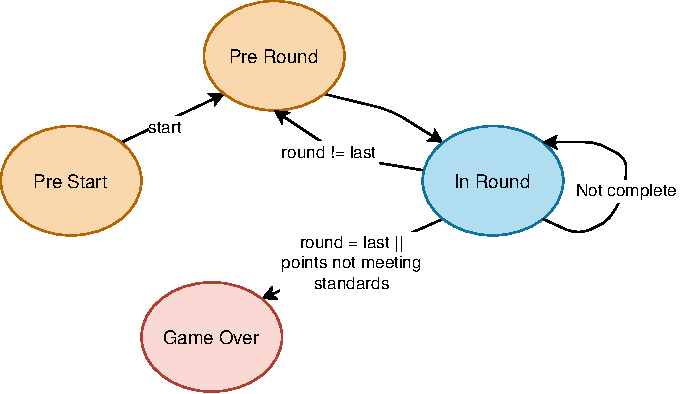
\includegraphics[width=0.5\textwidth]{res/img/primary-fsm.pdf}
  \caption{主状态机状态转换图}
  \label{fig:primary-fsm}
\end{figure}

Reset 后, 初始位于 Pre Start 状态, 当接收到 Start 信号后, 进入 Pre Round 状态. 
Pre Round 状态会给一些寄存器赋值, 以便于另一个状态机进行轮次配置. 在下一时钟周期即进入 In Round 状态. In Round 状态由另一个状态机
进行实现, 当状态机执行完毕后会判断当前轮次是不是最后一轮次, 如果是最后一轮次则直接进入
Game Over 状态, 然后判断当前分数是否达到进入下一轮次的条件, 若不满足也进入 Game Over 状态, 
否则进行下一轮次的配置, 并进入 Pre Round 状态.

下介绍 In Round 状态代表的次状态机. 如图 \ref{fig:secondary-fsm} 所示.

\begin{figure}[htbp]
  \centering
  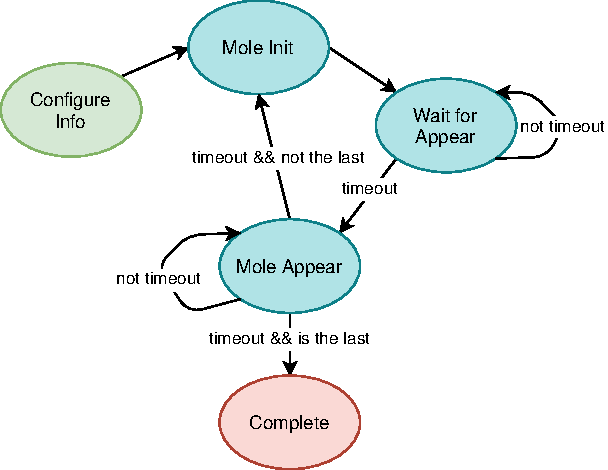
\includegraphics[width=0.5\textwidth]{res/img/secondary-fsm.pdf}
  \caption{次状态机状态转换图}
  \label{fig:secondary-fsm}
\end{figure}

次状态机控制游戏在一个轮次中的行为. 第一个状态为 Configure Info 状态, 该状态会根据当前轮次的配置
赋值给一些寄存器, 以便于后续的游戏逻辑. 该状态会在在每一轮次开始时执行一次. 随后进入 Mole Init 状态, 
Mole Init 状态会使用一个 LSFR 伪随机数发生器定义下一个地鼠显示前的时间, 随后进入 Wait for Appear 状态. 
该状态主要用于等待地鼠出现, 计时器计时结束后进入 Mole Appear 状态, 在该状态下会接收击打信号, 并判断是否击打成功.
计时器计时结束或击打成功后, 会判断当前地鼠是不是该轮次的最后一只地鼠, 若是最后一只地鼠, 则该状态机结束, 
回到主状态机. 

值得一提的是, 我在实现中广泛利用了参数化的思想. 我只需要在更改 Game Config 就可以自定义轮次数量, 
一个轮次中的地鼠数量以及地鼠出现前最短, 最长间隔时长, 地鼠每次出现的时长等等数据. 

\begin{lstlisting}[language=scala]
case class RoundInfo(
    val molesNum: Int,
    val points: Int,
    val appearTime: TimeNumber = 0.8 sec,
    val minTimeBeforeAppear: TimeNumber = 1 sec
) {
  def maxFloatingTime     = 3 sec
  def maxTimeBeforeAppear = minTimeBeforeAppear + maxFloatingTime
}
\end{lstlisting}

以上代码定义了一个轮次的基本信息. 在 \texttt{GameConfig} 类中有以下成员: 

\begin{lstlisting}[language=scala]
  val rounds: Seq[RoundInfo] = Seq(
    RoundInfo(3, 1, 4 sec, 1 sec),
    RoundInfo(5, 3, 2.5 sec, 1 sec),
    RoundInfo(7, 5, 1 sec, 1 sec)
  )
\end{lstlisting}
用于定义所有轮次的信息. 我只需要改这个成员的内容, 就可以实现参数化的游戏配置. 

\subsubsection{得分计数器}

得分计数器用于接收击打成功信号和当前轮次单个地鼠击打成功后增加的分数. 

得分计数器会输出两个 4 bits 数据, 分别代表十位和个位. 在硬件中直接实现十进制加法器
会消耗大量的硬件资源. 我们可以通过另一种方式规避直接实现十进制加法器. 

由于我们的时钟周期极快, 我们可以将要增加的分数放在一个 Buffer 中, 每周期 Buffer 中的分数
减 1 直到 Buffer 中的分数为 0. 当 Buffer 分数减 1 时, 实际的分数加 1, 这样我们就可以只
实现一个只支持每周期 +1 的十进制加法器, 从而减少了大量的硬件资源. 

\subsubsection{得分显示与轮次显示模块}

得分显示模块和轮次显示模块接收来自得分计数器和游戏控制器的信号, 将轮次和分数显示在屏幕上. 
我使用 32x16 的字模显示数字. 我将字模放在了 BRAM 中, 并将地址标签定为 \texttt{0x0}. 为了显示字符
\texttt{'/'}, 我将该字符的字模放在了理论上数字 10 应放置的地址(毕竟十进制没有数字10). 

\subsubsection{图层}

图层用于注册所有的 \texttt{Drawable} 信号的图像信息, 并进行仲裁, 从而输出当前像素应输出的真正的颜色.

注册的代码如下: 
\begin{lstlisting}[language=scala]
  def registerComponents(newComponents: List[_]) {
    newComponents.foreach {
      case c: Drawable     => {
        components += c.io.info
        c.io.hPos := io.hPos
        c.io.vPos := io.vPos
      }
      case c: GraphicsInfo => components += c
      case _               =>
    }
  }
  registerComponents(
    List(
      gameAreaBackground,
      scoreAreaBackground,
      io.molesGraphicsInfo,
      io.roundGraphicsInfo,
      io.scoreGraphicsInfo
    )
  )
\end{lstlisting}

仲裁的代码如下: 

\begin{lstlisting}[language=scala]
  io.rgb.foreach(_ := 0)

  for (c <- components) {
    when(c.visible) {
      io.rgb := c.rgb
    }
  }
\end{lstlisting}

非常简洁优雅, 且易于扩展. 

\subsubsection{VGA 驱动}

我采用的是 640x480(60Hz) 的时序. 该时序下像素时钟频率为 25.175 MHz, 我在实际上板时使用了
25 MHz 的像素时钟频率, 并直接将这个频率作为了游戏运行频率, 从而避免了跨时钟导致的复杂问题. 

VGA 的时序比较简单, 具体参数如下: 

\begin{lstlisting}[language=scala]
case class VgaConfig(
    hFrontPorch: Int = 16,
    hSync: Int = 96,
    hBackPorch: Int = 48,
    hActive: Int = 640,
    vFrontPorch: Int = 10,
    vSync: Int = 2,
    vBackPorch: Int = 33,
    vActive: Int = 480
)
\end{lstlisting}

\subsubsection{总成}

总成单元将我们自己实现的游戏部分和提供的按键驱动, VGA 转 HDMI 驱动相结合起来, 
用于上板操作. 同时我们需要在总成模块里例化时钟模块, 各种 BRAM 模块, 并进行 BRAM 
数据仲裁(根据地址标签). 

\subsection{仿真 -- 基于 C++ 的自编写可视化仿真工具}

随着计算机算力的增强以及硬件产品的不断, 出于敏捷开发的需要, 仿真工具也在不断发展.

这次的课程项目使用了复旦微电子开发的 FPGA 开发板, 但是由于板材有限, 同学之间共享
开发板的需求也很强烈, 因此我开发了一个基于 C++ 的仿真工具, 用于在没有开发板的情况下
对快速迭代的设计进行仿真.

\subsubsection{Verilator 简要介绍}

Verilator是一种用于 Verilog 硬件描述语言的开源仿真和验证工具. 它被广泛用于数字电路设计的功能验证和性能分析. 

Verilator的设计目标是提供高速仿真和验证, 以加快硬件设计的开发和验证过程. 相比于传统的基于事件驱动的仿真器, Verilator 采用了基于 C++ 的编译器前端技术, 将 Verilog 代码转换为高速的 C++ 仿真模型. 这种编译器前端方法消除了事件调度和时间轮询的开销, 提供了更高的仿真速度和性能. 

Verilator的工作流程包括以下步骤: 

\begin{itemize}
    \item 输入Verilog代码: Verilator接受Verilog代码作为输入,支持大部分IEEE-1364标准的Verilog语法. 
    \item 编译生成仿真模型: Verilator将Verilog代码转换为C++代码,并生成一个高速的仿真模型. 这个模型包含了与Verilog代码等效的硬件行为. 
    \item 编译仿真模型: 生成的C++代码通过常规的C++编译器进行编译,生成可执行的仿真模拟器. 
    \item 运行仿真: 生成的仿真模拟器可以加载测试向量或测试程序,并执行仿真过程. Verilator的仿真速度通常比传统的事件驱动仿真器快几个数量级. 
    \item 输出仿真结果: 仿真结果可以通过文本文件, VCD(Value Change Dump)文件或其他格式进行输出和分析. 
\end{itemize}

Verilator的优点包括:

\begin{itemize}
    \item 高速仿真:通过编译器前端技术, Verilator能够提供比传统仿真器更快的仿真速度, 加速硬件设计的验证过程. 
    \item 开源免费:Verilator是开源软件, 用户可以免费获取并自由修改, 分发. 
    \item 跨平台支持: Verilator 支持在多个操作系统上运行, 包括 Linux, Windows 和 macOS 等. 
    \item 集成测试环境: Verilator 可以与其他工具集成,如 GNU Make, SystemC 和 Python 等,提供更全面的测试环境和验证能力. 
\end{itemize}

\subsubsection{可视化仿真工具基本原理}

直接利用 HDMI 接口进行测试会带来很多麻烦, 例如, HDMI 需要两个时钟进行驱动, 但多时钟往往需要 PLL 等复杂的电路进行驱动, 
我们往往会调用 IP 核或者使用原语进行例化. 但这种方式对仿真并不友好, 我们甚至需要专门写一个模拟 PLL 行为的模块. 
同时, HDMI 协议较 VGA 更加复杂, 对仿真程序编写的要求更高, 性能也会因为转换器的存在而受到影响.

因此, 我们采用了一种更加简单的方式进行仿真, 游戏的主体部分采用 VGA 进行图像输出, 并在这一层进行仿真. 我们使用课程提供的
示例项目中的 Verilog 文件从 VGA转换为 HDMI, 在板上进行输出. 

我们使用 Qt 进行可视化界面的开发. 如图 \ref{fig:emulator} 所示, 界面上共有四部分组成. 

最上面是一个模拟的显示器, 用于从
Verilator 提供的接口获得 VGA 信号, 并将信号进行拼接, 存储成一个 \texttt{QImage} 对象, 并传递给界面显示主线程进行显示. 

中间的部分分别是一个 4x4 的键盘和两个按钮: Reset 和 Start. 通过点击按钮可以将信号传递到 Verilator 的接口中, 从而控制
游戏. Qt 提供了极为方便的信号与槽机制, 我们只需要 emit 按钮按下的信号到仿真线程, 仿真线程中就会对对应的
硬件接口进行赋值. 一个简单的实例如下: 

\begin{lstlisting}[language=c++, title={按下键盘按钮时发送信号}]
    connect(key, &Key::clicked, this,
            [this, key] { emit clicked(key_positions_.value(key)); });
\end{lstlisting}

\begin{lstlisting}[language=c++, title={仿真线程中的信号处理}]
auto HWDut::onKeyPressed(QPair<int, int> position) -> void {
  key_states_[position.first][position.second] = KeyState::Pressed;
  top_->io_keyPress = true;
  top_->io_keyIndex = position.first * 4 + position.second;
}
\end{lstlisting}

关于 VGA 信号接收与显示部分, 我使用了双缓冲技术. 为了降低线程之间交换数据的延迟, 从仿真线程到主界面线程我只传递了一个 \texttt{QImage*}
的指针. 仿真线程中的仿真类有两个 \texttt{QImage} 对象, 一个用于传递给主线程进行显示, 另一个则用于接收 VGA 信号并写入. 当一帧的数据全部
获取完毕时, 仿真线程会发送一个信号提醒主线程刷新帧, 并附带图像数据的指针. 仿真线程则需要交换两个 \texttt{QImage} 对象的指针的用途, 
这样就可以避免跨线程读取时的数据竞争.

每刷新一帧, 仿真器需要使硬件部分运行 $800 \times 525 = 420000$ 个时钟周期, 这对于仿真器来说是一个巨大的负担.
经过实验表明, 若不进行硬件实时仿真, 只运行 420000 次循环并像图像缓冲区中写入固定数据, 帧频率可以轻松达到百赫兹级别. 
但一旦开始进行实时仿真, 帧率就会急剧下降. 在 Debug 模式下只能达到 1-2 帧每秒, 而在 Release 模式下可以达到十几帧每秒.
因此, 我自己编写的代码部分并不是运行速度的瓶颈. 即使只能达到这样的速度, 对于我们快速迭代仿真也已经足够了. 

从 SpinalHDL 生成 Verilog 到 Verilator 重新编译 Verilog 文件, 我的全套仿真流程只使用 10s 就能完成. 由于是真正从硬件描述语言中
获得输出, 因此仿真的结果也是最真实的. 事实证明, 当我们的代码在仿真器中运行正常时, 在 FPGA 上也不会出现问题. 极大地减少了
调试的时间.

硬件编写不如软件代码编写那么便利, 工程师往往会使用大量的时间看波形, 定位错误, 并查找原因. 这种可视化仿真方法的出现, 
使得硬件编写也可以像软件编写一样快速定位错误, 而免去了大量的综合, 布局布线, 生成比特流的时间. 

\subsubsection{仿真波形图}

当然, Verilator 也可以生成 VCD 波形文件, 但是这种图像输出的设计, 会导致波形图文件极大, 在短短几秒就能达到几个G的大小.

图 \ref{fig:wave} 是输出一帧 VGA 信号的波形图. 

\begin{figure}
    \centering
    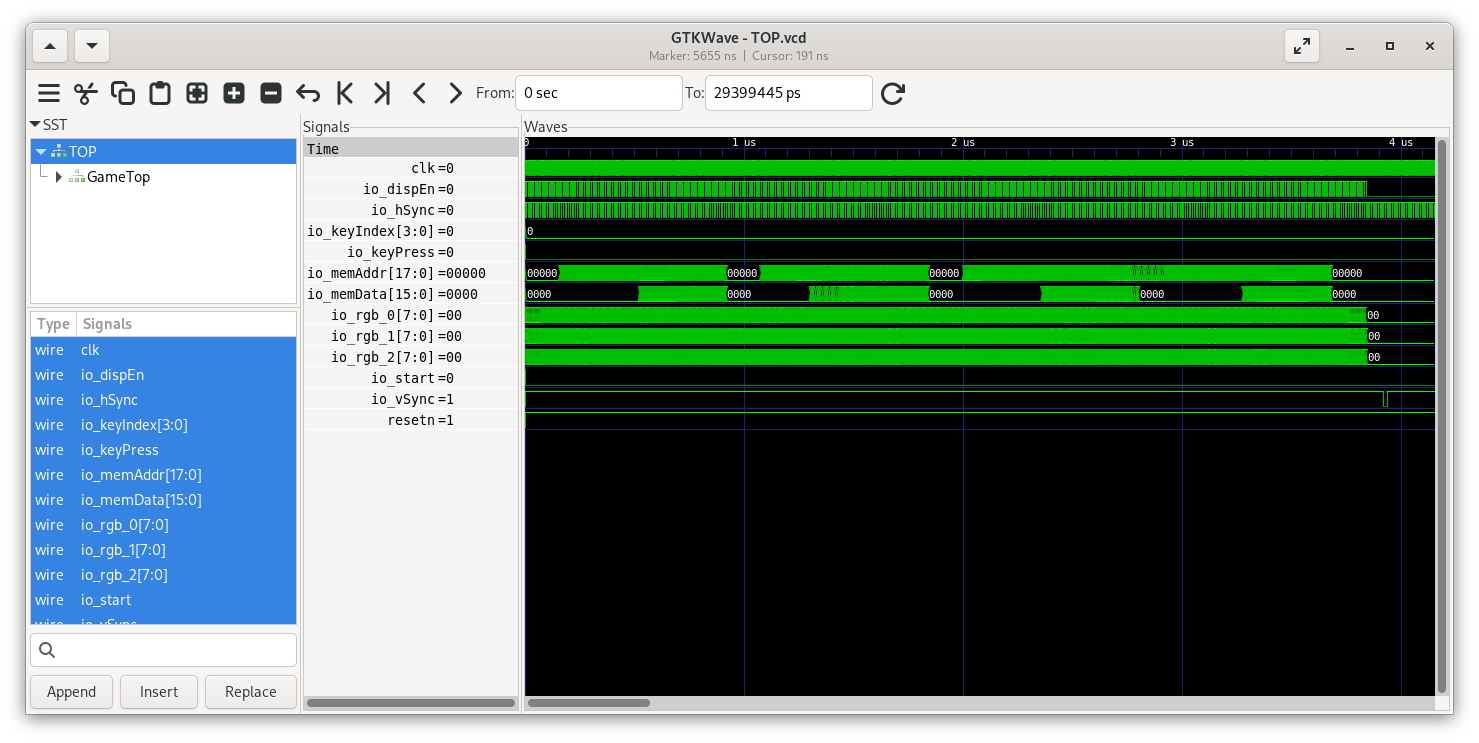
\includegraphics[width=\textwidth]{res/img/wave.png}
    \caption{仿真级主模块信号波形图}
    \label{fig:wave}
\end{figure}

可见, 行同步信号和场同步信号都表现正常. 由于这种方式调试过于复杂困难, 我基本没有采用直接看波形图的方法进行调试. 
而是使用我开发的仿真器进行模拟显示器的输出, 从而进行调试.

\subsection{COE 文件生成}

我采用了 Rust 语言用于将图片转化为 coe 文件, 以方便 Block Memory 
的实例化. 

\begin{lstlisting}[language=Rust]
fn write_coe(img: &DynamicImage, coe_path: &str) -> Result<(), Box<dyn std::error::Error>> {
    let (width, height) = img.dimensions();
    println!("Image dimensions: {}x{}", width, height);

    let mut data: Vec<u16> = Vec::new();
    for y in 0..height {
        for x in 0..width {
            let pixel = img.get_pixel(x, y);
            let r = (pixel[0] >> 3) & 0x1f;
            let g = (pixel[1] >> 3) & 0x1f;
            let b = (pixel[2] >> 3) & 0x1f;
            let a = (pixel[3] >> 7) & 0x01;
            let mut pixel: u16 = 0;
            pixel = pixel | (a as u16) << 15;
            pixel = pixel | (b as u16) << 10;
            pixel = pixel | (g as u16) << 5;
            pixel = pixel | (r as u16);
            data.push(pixel);
        }
    }

    let coe = Coe::new(coe_path, 16, height * width, data);
    coe.save()?;
    Ok(())
}
\end{lstlisting}

以上为生成 coe 文件的核心代码. 为了节约 FPGA 板上使用的 BRAM 资源, 我将一个ARGB像素用 16 位进行存储. 
其中, 最高位用于表示是否透明, 之后的 15 位依次存储红色, 绿色, 蓝色. 每一种颜色用 5 位进行存储.

在具体实现中, 我将两张 png 图片转换为了 coe 文件, 分别用于地鼠(隐藏)和地鼠(出现)的显示.

\subsection{综合与实现}

在 Procise 中建立工程后, 将所有设计的 RTL 文件导入到工程中, 并将顶层模块设置为 \texttt{top}. 
然后, 将 \texttt{top} 模块的输入输出端口与外部引脚进行绑定, 并设置时钟信号.

使用 Procise 成功完成综合布局布线并生成比特流流程后, 截图如图 \ref{fig:procise} 所示.

\begin{figure}[htbp]
  \centering
  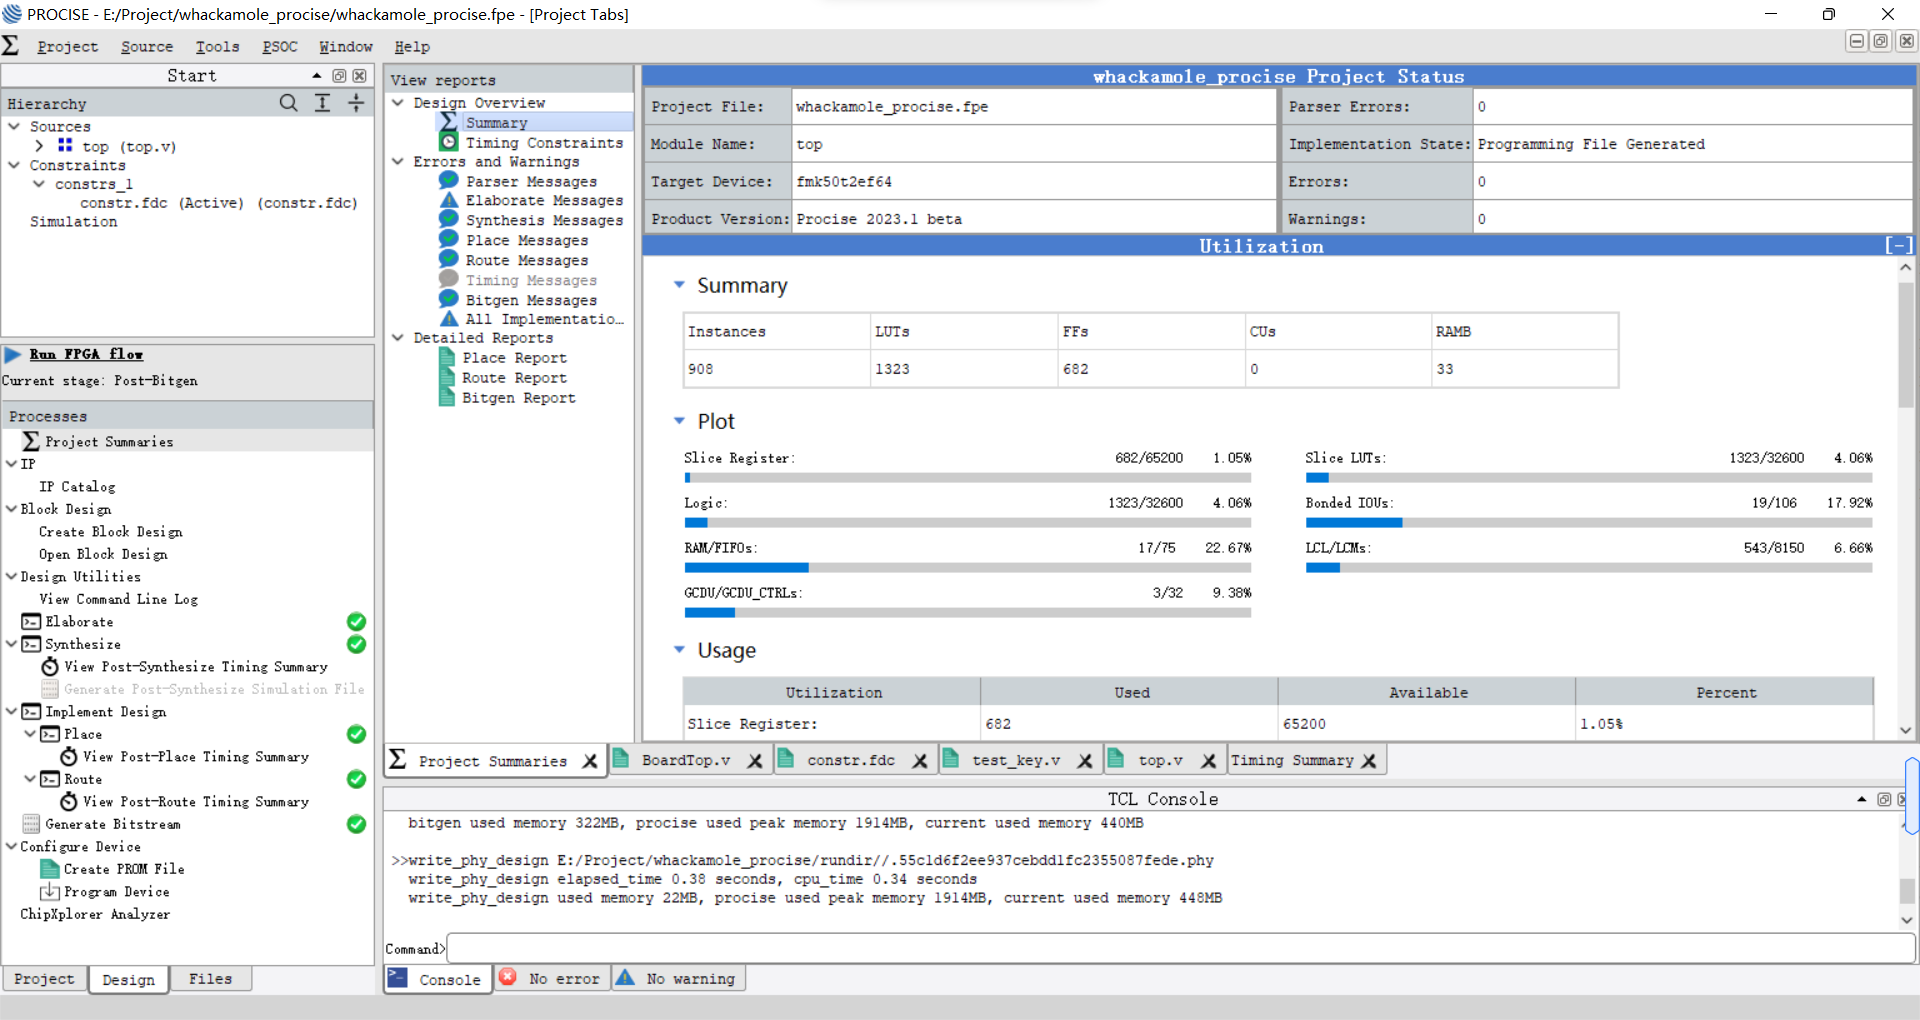
\includegraphics[width=\textwidth]{res/img/procise.png}
  \caption{Procise 使用截图}
  \label{fig:procise}
\end{figure}

\subsection{综合结果分析}

\subsubsection{资源利用分析}

Procise 完成布局布线后的资源利用统计如图 \ref{fig:resoucesuse} 所示. 

\begin{figure}[htbp]
  \centering
  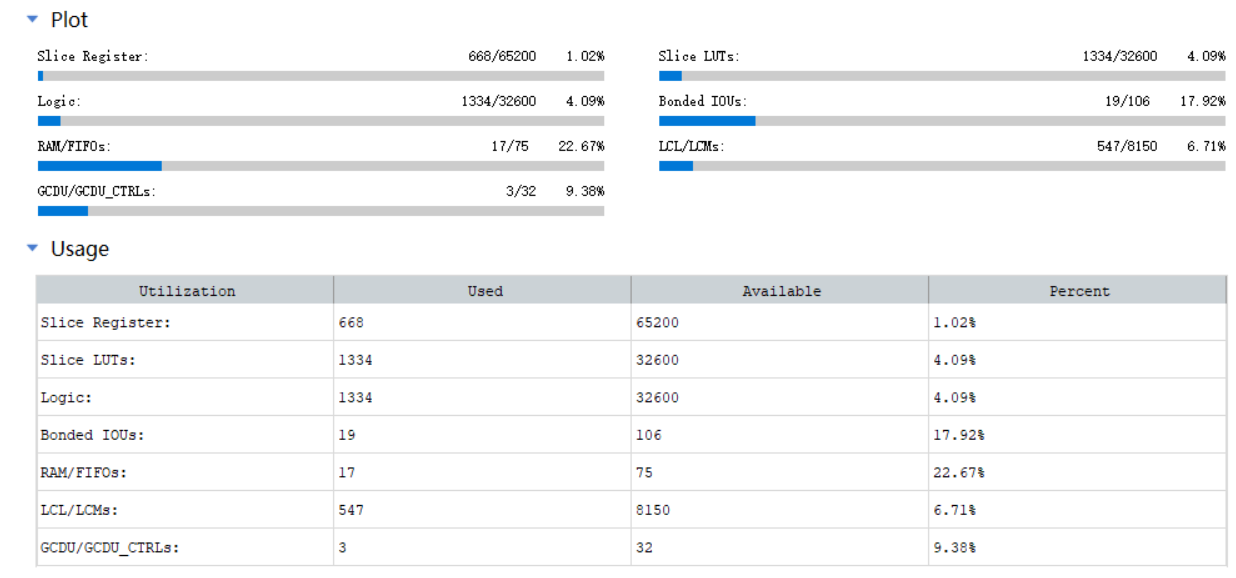
\includegraphics[width=\textwidth]{res/img/resouces_use.png}
  \caption{资源利用分析截图}
  \label{fig:resoucesuse}
\end{figure}

令我比较惊奇的是这块芯片的 BRAM 资源特别充足. 我使用过的
Xilinx Artix-7A35T 芯片只有 256Kbit 的 BRAM, 而根据手册, 这块芯片具有
2700 Kbit 的 BRAM 存储资源. 说明即使我不对图像信息进行压缩, 也可以将
所有的图像信息存储在 BRAM 中.

我的游戏逻辑并不复杂, 逻辑资源占用并不大, 这也得益于这款芯片的逻辑资源
非常丰富.

\subsubsection{时序分析}

时序分析结果如图 \ref{fig:timing}, 关键路径结果如图 \ref{fig:criticalpath} 所示.

25 MHz 频率下的时钟周期为 40 ns, 最差时序裕度为 16.7 ns, 说明可以在 25 MHz 的频率下正常工作.

\begin{figure}[htbp]
  \centering
  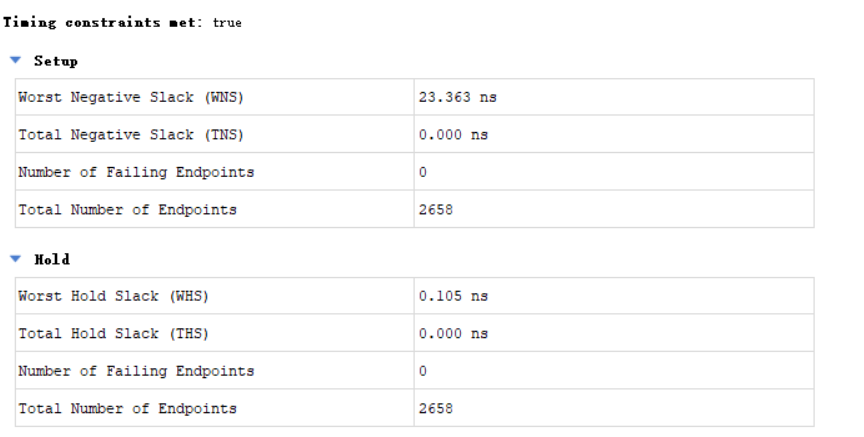
\includegraphics[width=\textwidth]{res/img/timing.png}
  \caption{时序分析截图}
  \label{fig:timing}
\end{figure}

\begin{figure}[htbp]
  \centering
  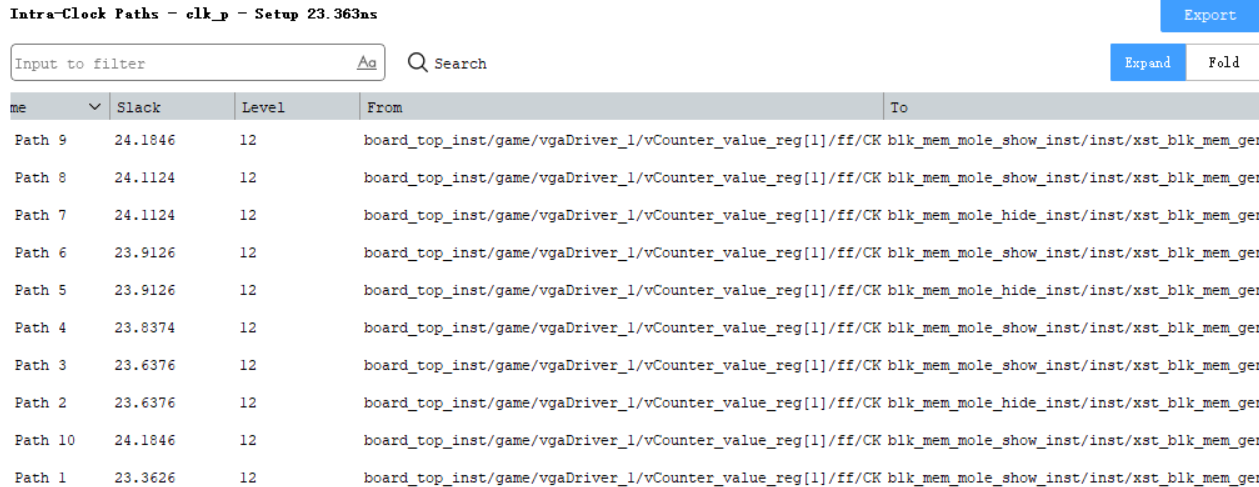
\includegraphics[width=\textwidth]{res/img/criticalpath.png}
  \caption{关键路径分析截图}
  \label{fig:criticalpath}
\end{figure}

\subsection{下载测试}

上板测试截图如图 \ref{fig:game} 所示.

\begin{figure}[htbp]
  \centering
  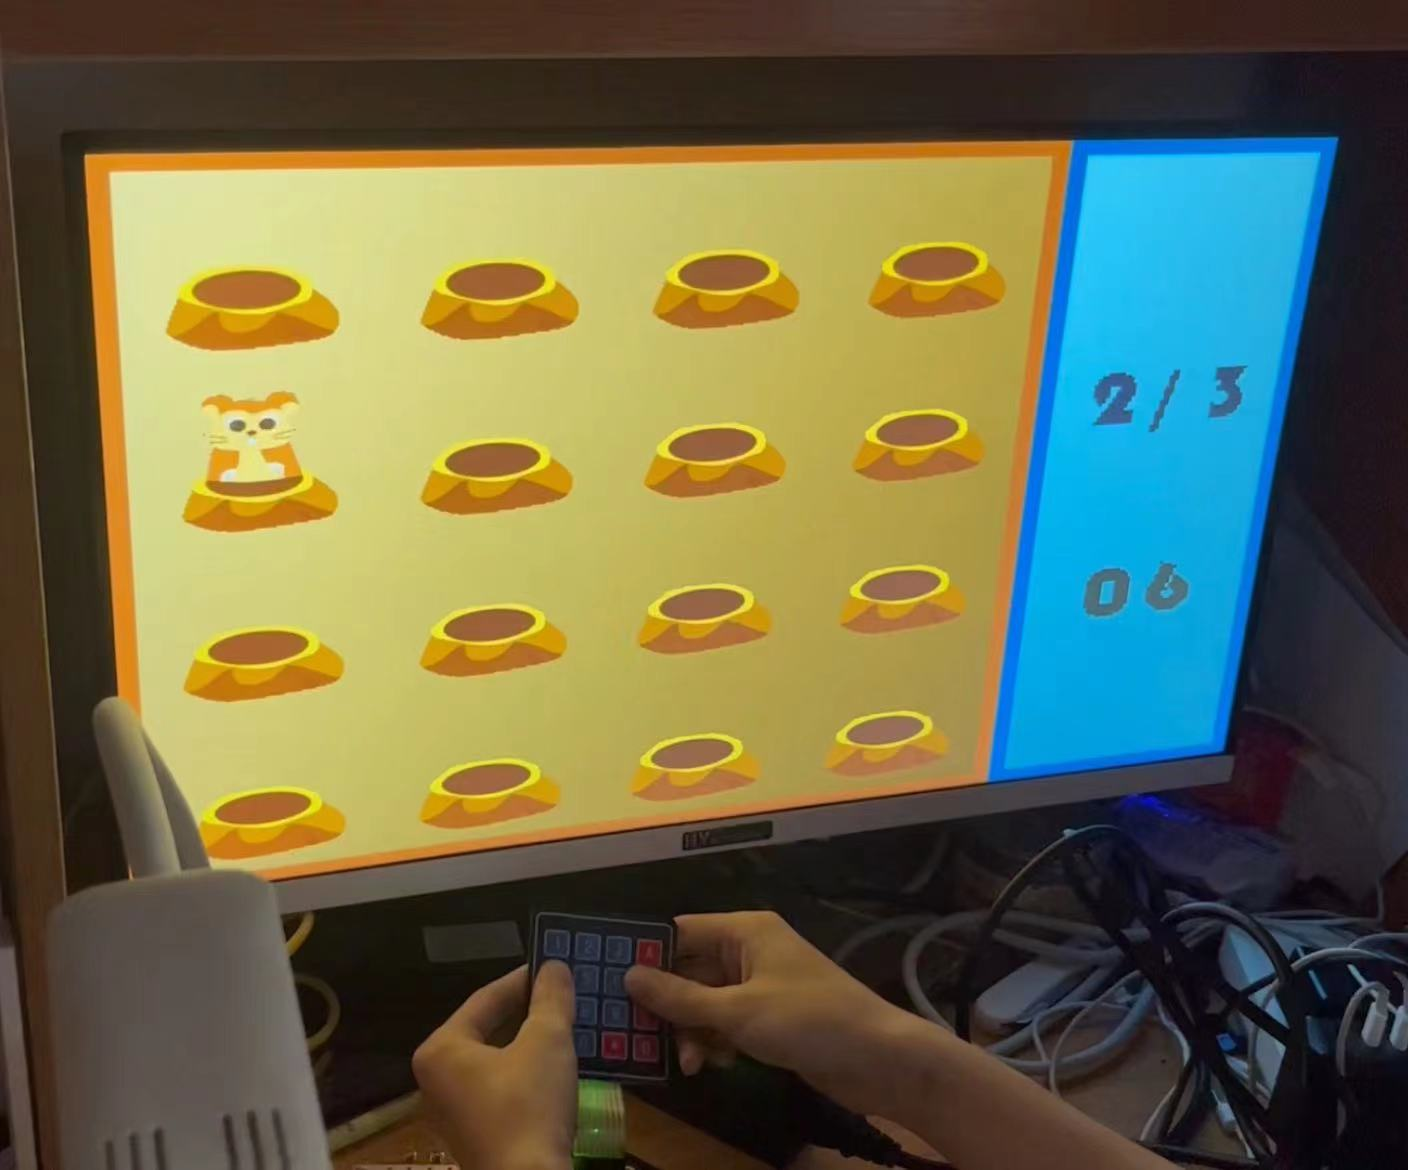
\includegraphics[width=0.8\textwidth]{res/img/validation.jpg}
  \caption{上板测试截图}
  \label{fig:game}
\end{figure}

运行正常, 并且与图形化仿真一致. 说明我的设计没有问题.

\section{设计总结}

\subsection{注意事项与编程技巧}

\subsection{心得体会}

\subsection{总结}

\appendix

\section{主要文件列表}

\begin{table}
\caption{主要文件列表}
\centering
\begin{tabular}{lll}
    \toprule
    \heiti 文件名 & \heiti 路径 & \heiti 说明 \\
    \midrule
    \texttt{main.scala} & \texttt{src/main/scala} & 主文件 \\
    \bottomrule
\end{tabular}
\end{table}


\end{document}
